\documentclass[paper=a4, fontsize=11pt]{scrartcl}
\usepackage{enumerate}
\usepackage{amsmath}
\usepackage{amssymb}
\usepackage{tikz}
\newcommand{\parens}[1]{ \left( #1 \right) }
\begin{document}
\noindent Willy Xiao and Kevin Eskici \\ STAT 221 \\Pset 4\\ Nov 4, 2014
\begin{enumerate}[\text{question }1.]
  \item
    \begin{enumerate}[1]
      
      \item   
      $p(\lambda, \theta) \propto \lambda^{-1}$\\
      $\begin{bmatrix} N \\ \theta \end{bmatrix} = f\parens{\begin{bmatrix} \lambda \\ \theta \end{bmatrix}}$\\
      $p(N, \theta) = p(\lambda, \theta) * \begin{Vmatrix}  \frac{\partial \lambda}{\partial N} &  \frac{\partial \theta}{\partial N} \\ \frac{\partial \lambda}{\partial \theta} &  \frac{\partial \theta}{\partial \theta} \end{Vmatrix}$\\
      Our Jacobian is $\begin{vmatrix} \theta & {-\lambda N^{-2}} \\N & 1 \end{vmatrix}$\\
      and its determinant is $\theta + \frac{\lambda}{N}$\\\\
      $p(N, \theta) \propto \frac{1}{\theta N} * (\theta + \frac{\lambda}{N})$\\
      $= \frac{1}{\theta N} * (\theta + \frac{\theta N}{N})$\\
      $= \frac{2}{N}$\\
      $\propto \frac{1}{N}$
      \\This prior favors smaller values of N.

      \item It is an improper prior: $\int_0^\infty{\int_0^1{\lambda^{-1}}}d\theta d\lambda \rightarrow \ln(\infty) - \ln(0)$. This cannot integrate to 1 with any constant factor.
	
	\item No $p(\lambda, \theta)$ is not a non-informative prior in the sense of Jeffreys.\\ 
	$p(y_i| \theta, \mu) = \frac{(\theta \mu)^{y_{i}}}{y_{i}!} e^{-\theta \mu}$\\
	$y_i log(\theta | \mu ) - log({y_i}!) - \frac{\theta}{\mu}$\\
	$\frac{\partial I}{\partial \theta} = y_i (\theta \mu)^{-1} \mu - \frac{1}{\mu} = 
	y_i (\theta)^{-1} - \frac{1}{\mu}$\\
	$\frac{\partial I}{\partial \mu} = y_i \mu + \theta \mu^{-2}$	\\
	$\frac{\partial^2 I}{\partial \theta^2} = -{y_i}\theta^{-2}$\\
	$\frac{\partial^2 I}{\partial \mu^2} = y_i - 2\theta \mu^{-3}$\\
	$\frac{\partial^2 I}{\partial \mu \partial \theta} = \mu^{-2}$\\
	$\frac{\partial^2 I}{\partial \theta \partial \mu } = \mu^{-2}$\\
	This gives us the fisher's information matrix $\begin{pmatrix}-{y_i}\theta^{-2} & \mu^{-2} \\\mu^{-2} & y_i - 2\theta \mu^{-3} \end{pmatrix}$, which has determinant $({y_i}\theta^{-2})^2 - 2\theta \mu^{-3}y_i - \mu^{-4}$, the square root of which is not proportional to $\frac{(\theta \mu)^{y_{i}}}{y_{i}!} e^{-\theta \mu}$.


	
	\item See R code and MCMC design note. Also figures 1 and 2 show posterior contours for an impala and waterbuck chain (2 were chosen arbitrarily, but they all look similar). Figures 3 and 4 are additional diagnostic plots for one of the impala chains-autocorrelation and mixing look good. To run diagnostics on other chains, just load the corresponding chain in $checkdiagnostics.R$ and run the script (note the R datafiles for chains are not included due to space constraints but will be generated when you run the slurm job).
	
	\item Posterior for N\\
	$\int^1_0 \parens{\prod_{i=1}^n\binom{N}{x_i}\theta^{x_i}(1-\theta)^{N - x_i}}* \frac{1}{N} d\theta$\\
	$=\int^1_0 \parens{\prod_{i=1}^n\binom{N}{x_i}}\theta^{\Sigma x_i}(1-\theta)^{nN - \Sigma x_i}* \frac{1}{N} d\theta$\\
	$= \frac{1}{N} \int^1_0 \theta^{\Sigma x_i}(1-\theta)^{nN - \Sigma x_i}\prod_{i=1}^n\binom{N}{x_i} d\theta$\\
	$= \frac{1}{N} \prod_{i=1}^n\binom{N}{x_i}  \int^1_0 \theta^{\Sigma x_i}(1-\theta)^{nN - \Sigma x_i}d\theta$\\
	If we define $S = \Sigma x_i$, the integral above has the form of a\\ 
	Beta($\alpha=S+1, \beta=nN - S + 1$ ) pdf\\
	Using this we get, $\frac{(nN-S)!}{(nN + 1)!N)}$, which when $n=1$, $\rightarrow \frac{x_i}{N(N+1)}$\\\\
	Using our function $find.norm.log.const$ defined in $keskici\_wxiao\_ps4\_post.R$, we found that the normalizing constant for the impala dataset was $e^{15.63617}$ and the normalizing constant for the waterbuck dataset was $e^{16.83744}$. Figures 5 and 6 show the posteriors for Impala and Waterbuck respectively.
	
	\item Give POSTERIOR PROBS N $>$ 100
      
    \end{enumerate}
    
    Note about MCMC Design:
\end{enumerate}

\clearpage
Appendix: \\
\begin{figure}[h!]
  \caption{Countour plot for 8th Impala Chain}
  \centering
	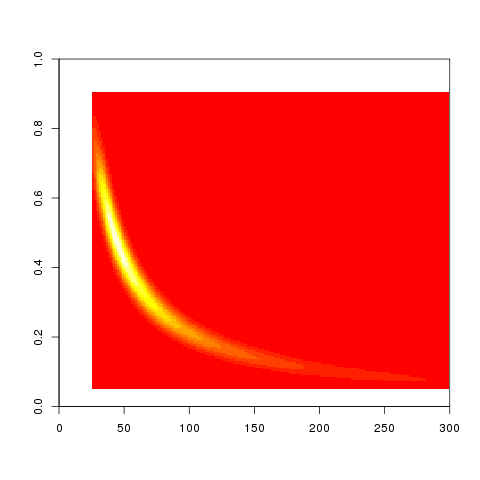
\includegraphics[scale=.8]{keskici_wxiao_ps4_task_impala_run5_plot8.png}
\end{figure}

\begin{figure}[h!]
  \caption{Countour plot for 5th Waterbuck Chain}
  \centering
	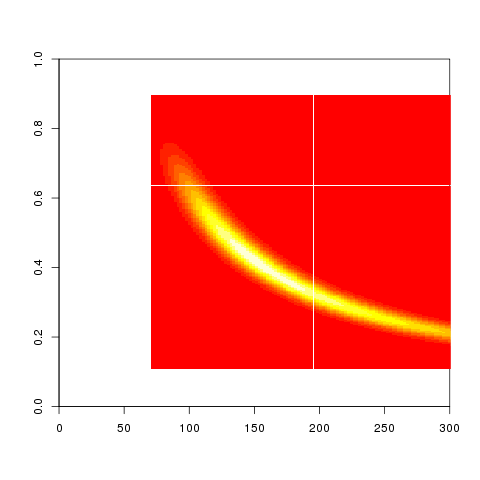
\includegraphics[scale=.8]{keskici_wxiao_ps4_task_waterbuck_run5_plot5.png}
\end{figure}

\begin{figure}[h!]
  \caption{Trace plots for 8th Impala Chain}
  \centering
	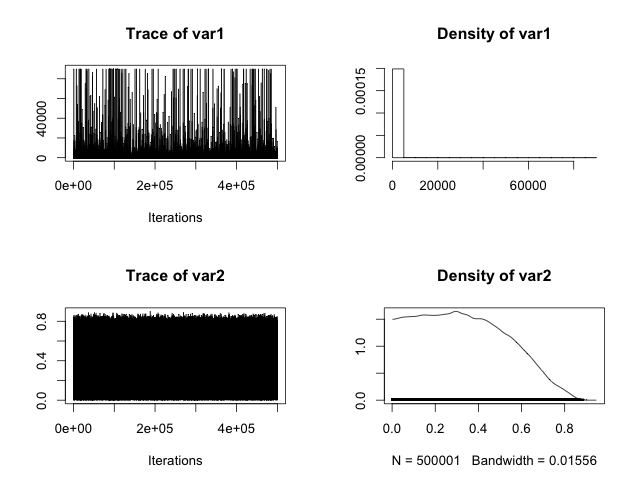
\includegraphics[scale=.8]{Rplot_job8a.png}
\end{figure}

\begin{figure}[h!]
  \caption{Autocorrelation plot for 8th Impala Chain}
  \centering
	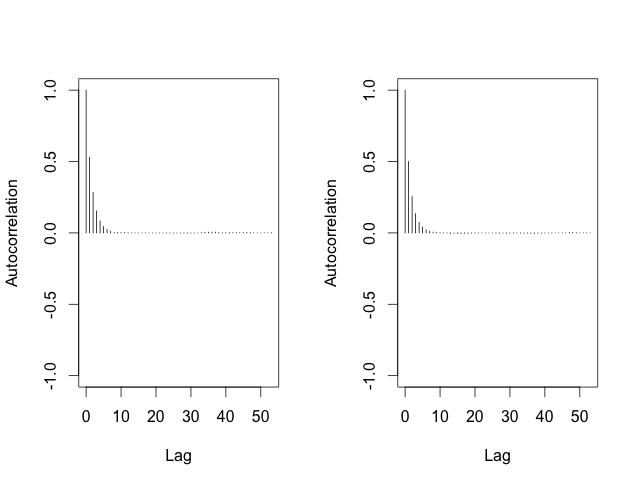
\includegraphics[scale=.8]{Rplot_job8b.png}
\end{figure}

\begin{figure}[h!]
  \caption{Posterior for Impala Dataset}
  \centering
	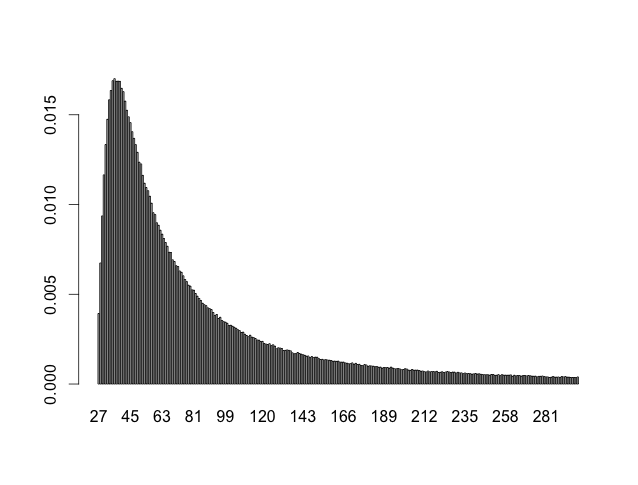
\includegraphics[scale=.8]{impala.png}
\end{figure}

\begin{figure}[h!]
  \caption{Posterior for Waterbuck Dataset}
  \centering
	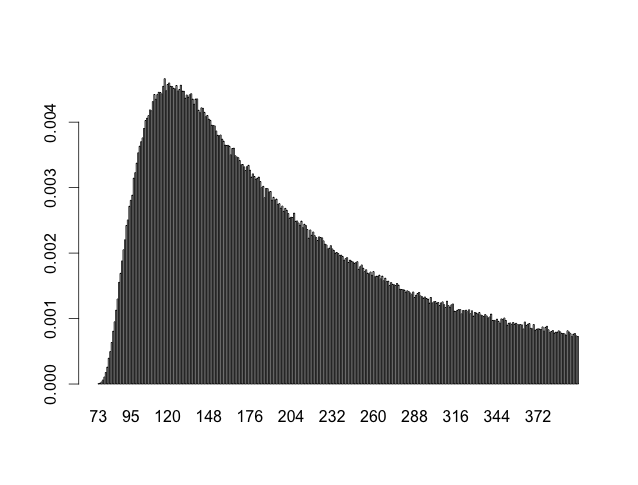
\includegraphics[scale=.8]{waterbuck.png}
\end{figure}

\end{document}
